

Popsat termín BigData není úplně snadné, a to hned z několika důvodů. Především proto, že neexistuje žádná přesná definice tohoto pojmu. Tento termín je stejně jako obor, kterého se týká, velice dynamický a rychle se mění. K obtížnější definici pojmu přispívá také fakt, že se hojně používá v marketingové komunikaci jako tzv. \uv{Buzzword} za účelem vzbudit zájem čtenáře/posluchače, přestože může být použit v nesprávném kontextu.

Termín BigData označuje manipulaci s datasety tak velkými, že je nemožné nebo velice obtížné s nimi manipulovat za pomocí tradičních nástrojů a databází (převážně relačních). Pod pojmem manipulace s datasety myslíme:

\begin{itemize}
  \item Sběr
  \item Organizace
  \item Ukládání
 \item Prohledávání
 \item Sdílení
 \item Analýza
 \item Vizualizace
\end{itemize}

Nalezení této hranice, či její přesná definice, je komplikovanější problém mimo rozsah této práce. Na toto téma již bylo publikováno mnoho jiných prací. Jak jsem zmínil již v úvodu, práce se dále také nezabývá porovnáním BigData a klasických relačních databází. 

V této kapitole se pokusím obecně přiblížit, co to tedy BigData jsou, jak se liší a důvod vzniku tohoto odvětví.


\section{Trend velkých datasetů}
Jak jsem již naznačil, BigData se věnují zpracování velkých datasetů. Trend upřednostňování velkých datasetů oproti několika menším, které v součtu mají stejný objem a nesou stejné množství informace, začal vzhledem k jednoduššímu hledání a objevení i zdánlivě neexistujících korelací, projevení obchodních trendů, či určování určitých jevů v reálném nebo skoro reálném čase. % Nerozumim větě % 

\section{3V}
Jak naznačil předchozí odstavec, BigData nejsou pouze o objemu zpracovávaných dat, jak by se na první pohled mohlo zdát. Jedná se o komplexnější kategorizaci, kde hrají roli i ostatní charakteristiky, které se v literatuře značí zkratkou 3V, odvozenou od počátečních písmen těchto kategorií v anglickém jazyce. 

\begin{figure}[h]
\centering
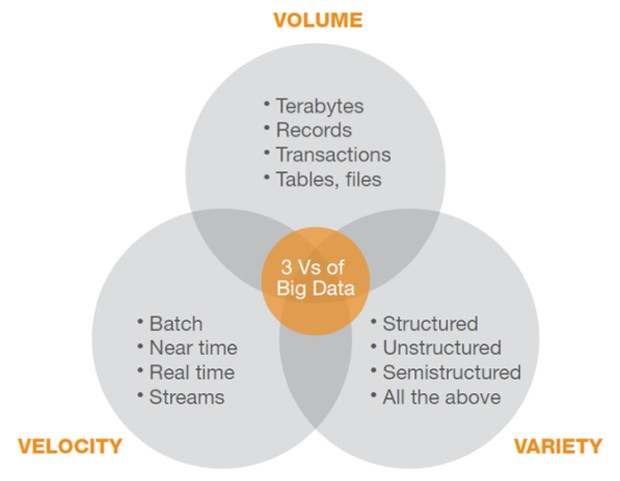
\includegraphics[scale=0.6]{images/3v}
\caption{http://smartdatacollective.com/yellowfin/75616/why-big-data-and-business-intelligence-one-direction}
\label{fig:3v}

\end{figure}

\subsection[3v-volume]{Obsah (Volume)}
Data se dnes zdaleka nevyskytují jen v textové podobě, můžeme je uchovávat formou hudby, obrázku či videa. Vzhledem k tomuto faktu čelíme exponenciálnímu nárůstu množství uchovávaných dat a není výjimečné, aby enterprise systémy uchovávaly terabyty nebo petabyty dat. Data tedy tvoří množství informací, které je dost často vyhodnocováno z různých úhlů a následně uloženo a znovu vyhodnocováno, a přestože původní data zůstala nezměněna, díky reevaluaci nám jejich množství roste závratným způsobem. Tímto způsobem může být na objem nahlíženo jako na jednu z charakteristik. % charakteristik čeho? %

\subsection{Rychlost (Velocity)}
Na rychlost můžeme nahlížet hned ze dvou pohledů. Prvním pohled vyjadřuje rychlost, jakou nám data přibývají a jak aktuální pro nás jsou. Například historie vývoje měnového kurzu je informace, jejíž včerejší hodnota je naprosto nevypovídající a mění se s každou minutou. Změnila se i rychlost, jakou noviny a televizní stanice získávají informace skrze sociální sítě. Objem dat tedy roste rychle a aktuálnost informací se rapidně zkrátila. Druhý pohled na tuto charakteristiku se zabývá rychlostí, jakou data potřebujeme zpracovávat. Jsou informace, které k nám proudí velice často (například každou minutu), ale jejich vyhodnocení dává smysl ku příkladu jen jednou za 24 hodin. Ovšem jsou také data, které potřebujeme zpracovávat v reálném čase, tak, jak k nám proudí. Dobrým příkladem takových dat mohou být akutální informace z meteorologické stanice. 
Rychlost, v jaké jsou dnes data zpracovávána, se mnohonásobně zmenšila a tedy nejen objem dat, ale i rychlost zpracování reprezentuje samotná BigData.

\subsection{Různorodost (Variety)}
Jak je z Obrázku ~\ref{fig:3v} patrné, různorodost dat znamená jejich strukturovanost/nestrukturovanost. Již bylo zmíněno, že data mohou mít mnoho podob. Ale i data ve stejné podobě (například textové), mohou být jinak strukturována a tomuto faktu je potřeba se přizpůsobit a uchovávat a zpracovávat data v jiných formátech. % Proč? %
Různorodost a adaptabilita jsou tedy posledními charakteristikami BigData.

\section{BigData zjednodušeně}
Předcházející řádky by měly sloužit jako shrnutí a lehký úvod do problematiky BigData. Dalo by se vlastně také říci, že BigData nejsou jen o velkém množství dat, ale je to celý koncept uchovávání a možností nových náhledů na stávající data, ale také návod, jak zachytit a zpracovat budoucí data. Další odstavce budou věnovány historii tohoto konceptu, ale také nejtypičtějších odvětví, kde se s ním můžeme setkat. 

\section{Historie}

Již od počátků počítačové éry bylo potřeba data analyzovat. \cite{history} S rychle se zvyšující dostupností moderních technologií a jejich obecnému přijetí ve společnosti, se posouvaly hranice této potřeby od vládních organizací až po současnost, kdy obrovské množství informací a jejích analýzu potřebují i malé podniky.

\subsection{30. a 40. léta}
V této době se používaly první počítačové simulace. Prim hrálo především válečné odvětví, kde například vědci z projektu Manhattan pomocí počítačových simulací simulovali dopad a následný zničující efekt jaderné bomby.

\subsection{50. a 60. léta}
V tomto období se počítače (a s nimi také zpracování a analýza dat) rozšířily do velkých korporací a výzkumných laboratoří. Počítač ENIAC například generoval první modely pro předpověď počasí. Analytici také vyřešili první problém nejkratší cesty a mnoho dalších, viz. také \cite{history}.

\subsection{70. až 90. léta}
V této době se analytická činnost rozšířila o středně velké podniky a technologické startupy. Objevují se také dnes již dobře známé případy užití. Dobrým příkladem takových případů je třeba první predikční model na pokles a růst akcií. Dále také stojí za zmínku první komerční nástroj pro modelově řízené rozhodování. Důležitým milníkem je rovněž vznik společností, jako je Ebay a Amazon. Bitva o personalizaci online nákupů právě začala! Google implementuje první vyhledávací algoritmus, který zvyšuje relevanci výsledků.

\subsection{2000 až součanost}
V tomto období se analytika rozšířila až na oblast malých podniku a analytických expertů (jednotlivců). Začíná mít obrovský dopad na život každého z nás. Samozřejmostí začínají být dynamické změny cen zboží, doporučování produktů, hudby a filmů nebo řízení dopravy. Rozvíjejí se obory, jako je analýza a procesování přirozeného jazyka z novin, e-mailů nebo sociálních sítí. Příchodu BigData, vzhledem k levné dostupnosti výpočetního výkonu a rychlosti zpracování dat, již nic nestojí v cestě.

\subsection{Budoucnost}
Předpokládá se, že v budoucnu bude analytická činnost řídit každodenní rozhodování i na úrovni jednotlivců. V běžném životě se přínos analýzy dat projeví například: Predikce v policejní sféře a boji proti zločinu, výzkum ve zdravotnictví nebo kompletně personalizovaná zákaznická interakce i pro malé podniky a řetězce. % seznam? %

\section{Nástup sociálních sítí}
Big Data zažila obrovský nástup také díky příchodu a masivnímu rozšíření sociálních sítí, a to hned ze dvou důvodů. Prvním důvodem je, že nástup sociálních sítí přilákal tisíce výzkumníků, kteří začali sbírat data z Facebooku a Twitteru. Tito výzkumníci následně hledali různá spojeni mezi zprávami a účty, z kterých poté vyvozovali závěry ohledně těchto sociálních sítí. Další možností, k čemu vytěžená data používali, bylo vytváření tzv. sociálních grafů. Historicky sbírali antropologové a sociologové data o lidských vztazích skrze dotazníky, rozhovory, pozorování a experimenty. Dolováním dat ze sociálních sítí, kde lidé sdílejí mnoho detailů ze svých životů, se jim otevřel nový kanál, kde mají všechny tyto informace jednoduše k dostání a stačí je pouze analyzovat.

BigData podle vědců představují 2 druhy sociálních sítí: \uv{Artikulované sítě} a \uv{Behaviorální sítě}. První kategorie znázorňuje sítě, kde uživatelé zadávají svá přátelství a konexe skrze technické mechanismy jako například: telefonní seznamy, emaily, seznamy přátel z jiných sití atd. Druhou kategorií jsou sítě odvozené od komunikačních vzorců. Do této skupiny spadají uživatelé, kteří si píšou zprávy nebo jsou označení na společných fotkách. Obě tyto skupiny mají pro výzkumníky velký význam, přestože jím nepřikládají takovou váhu jako reálným osobním vztahům. \cite{social} % je ta první věta správně? %

Druhým důležitým aspektem, proč jsou sociální sítě pro BigData důležité, je fakt, že tyto sítě samy potřebují někde svá data uchovávat a zpracovávat. Technologické týmy stojící za těmito službami se tak ve značné míře podílejí jako kolaborátoři na BigData projektech, či dokonce vytvářejí a následně uvolňují svoje technologie k užití pro širokou veřejnost. Pro komunitu jsou důležité i přednášky a prezentované poznatky od těchto datových gigantů, kteří prozkoumávají a prolamují lidstvu dosud známe bariéry a umožňují tím využívání technologických pokroků i jiným subjektům. 

Sociální sítě samozřejmě nejsou jediným průkopníkem na poli BigData. Internetoví giganti jako Google, Amazon a Yahoo přispívají neméně výrazným dílem. Na sociálních sítích je však zajímavé to, že jejich data jdou do jisté míry jednoduše dolovat, díky čemuž vzniklo mnoho spolčeností, které se začaly jejich analýzou a sběrem zabývat a způsobily tím popularizaci spojení BigData se sociálními sítěmi. 


\section{Odvětví}

Jak již bylo zmíněno v předchozí sekci, v dnešní době můžeme na BigData narazit kdekoliv. Zde bych chtěl poukázat na široké spektrum využití napříč různými činnostmi, kterými se lidstvo zaobírá.\cite{sektory}

\subsection{Maloobchod}
Péče o zákazníka a samozřejmě také zvýšení zisku jsou hlavními motivy pro zpracovávání a analýzu dat. Na základě chování uživatelů (aktivita na webu, zákaznická karta, anonymní zákazníci) můžeme předpovídat chování zákazníka v každém stádiu nákupu. Toto chování lze navázat také na podniková data a hledat korelace pomocí Map Reduce mechanismů. Největším průkopníkem spojování BigData a maloobchodu je bezesporu řetězec Tesco se svou věrnostní kartou ClubCard. Na základě zákazníkovy nákupní historie sestavují žebříček produktů k doporučení, či dokonce dokáží odhadnout období těhotenství svých zákaznic.\cite{tesco}

\subsection{Věda a výzkum}

Není žádným překvapením, že ve vědě a výzkumu se využívají BigData na uchovávání výsledků z měření či pro hledání korelací v naměřených hodnotách. Držitel Nobelovy ceny Peter Higgs používal NoSQL databázový systém Cassandra na zpracování svých dat, díky nímž prokázal existenci tzv. Higgsova Bosonu \cite{higgs}.

\subsection{Meteorologie}
Díky sběru a vyhodnocování dat z meteorologických stanic se podařilo vytvořit mnohem spolehlivější a přesnější modely pro předpovědi počasí, a to jak dlouhodobých, tak také krátkodobých. 

\subsection{Finance}
Ve finančním sektoru je způsobů využití hned několik. Například již výše zmíněné doporučování produktů dle historie transakcí a sběru  osobních dat. Banky a jiné finanční instituce podobným způsobem nabízejí zákazníkům vhodné finanční produkty, jako jsou například hypotéky. Mnohem zajímavějším případem využití BigData je detekce podvodů, kdy jsou banky na základě analýzy všech transakcí schopny hledat vzory podvodných chování a vyhodnotit určité transakce jako podezřelé a tím tak chránit své klienty nebo samy sebe.

\subsection{Webová optimalizace}
Na základě ukládání a následného zpracování veškerého chování uživatele na stránce mohou firmy optimalizovat webové stránky a jejich obsah, či ho případně restrukturalizovat. Po vyhodnocení chování konkrétních uživatelů je možné jim obsah stránky automaticky personifikovat a podsouvat tak uživatelům pro ně zajímavé věci, aniž by se k nim museli složitě proklikávat.

\subsection{BioInformatika}
V bioinformatice se BigData využívají například k mapování genomů nebo k sekvenční analýze. Tyto informace pomáhají k lepšímu pochopení DNA a také k prevenci genetických poruch a vrozených nemocí či k usnadnění jejich léčby. \cite{industries} 

\section{Dnešní možnosti}
V dnešní době existují v podstatě 3 možnosti jak začít s BigData. 

\subsection{Specializované firmy a hotová řešení}
Na internetu nalezneme několik firem zabývajících se analýzou vašich dat, kde veškerá analýza a vizualizace probíhá v softwaru třetí strany. Mezi nejznámější patří společnost Good Data \cite{gooddata}. Tyto firmy se však specializují na zpracování firemních dat a vizualizaci v jejich vlastních BI nástrojích.

\subsection{Hotová enterprise řešení}
Další možností je vybrat nějaké komplexní řešení od firem zabývajících se platformou BigData, které vám dodají software pro ukládání, analýzu a vizualizaci vašich dat. Programování komponent či jejich konfigurace je v režii zákazníka a tyto firmy poskytují licence, školení a technickou podporu. Tuto možnost poskytuje například IBM.

\subsection{Open Source a řešení z něj vycházející} 
Poslední možností je použití Open Source nástrojů, které umožní ukládat, analyzovat a vizualizovat data. Toto je cesta, kterou jsem se vydal v rámci této práce a budu se jí tak nadále věnovat. Drobnou nadstavbou těchto řešení mohou být firmy nabízející komerční balíčky těchto Open Source řešení. Jedná se o velice populární přístup v případech, kdy je potřeba zkombinovat několik nástrojů dohromady. Jejich konfigurace bývá velice obtížná, a proto tyto komerční balíčky nabízí již nakonfigurovaná hotová řešení většinou i s drobnou nadstavbou, která umožňuje provádět některé nadstandardní procesy a činnosti. 
